\begin{figure}[h]
    \centering
    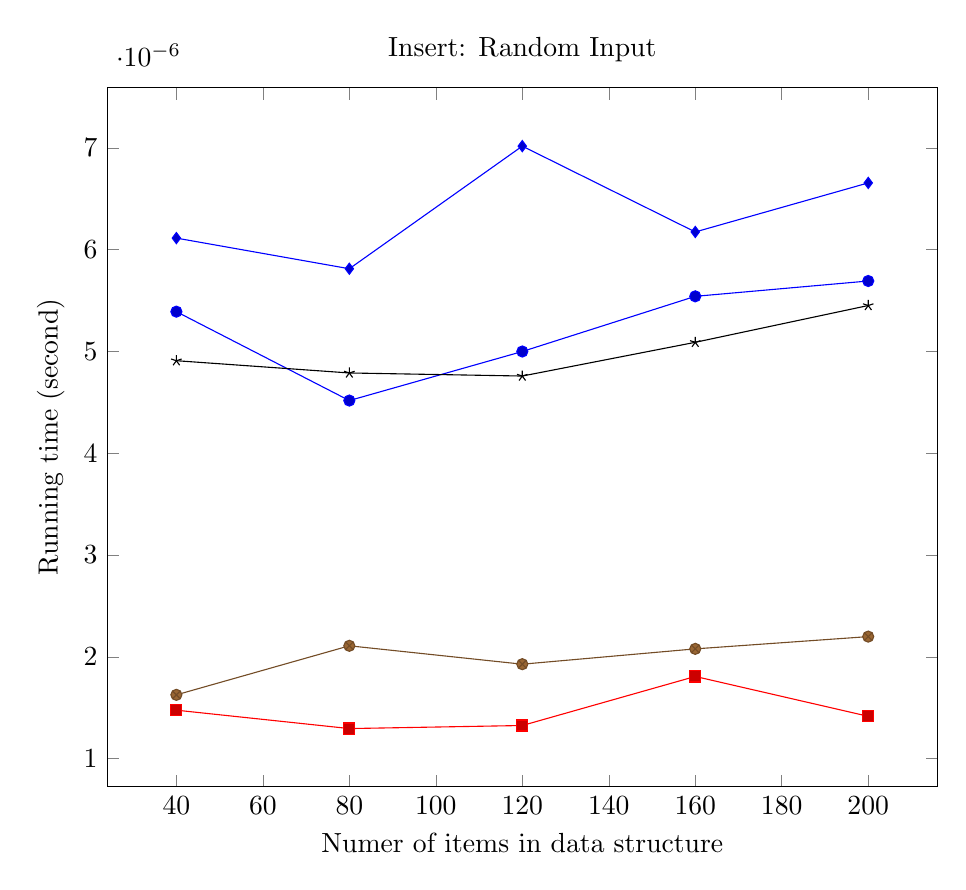
\begin{tikzpicture}
        \begin{axis}[
            xlabel={Numer of items in data structure},
            ylabel={Running time (second)},
            title={Insert: Random Input},
            width=\textwidth
        ]
		\addplot coordinates {
			(40, 5.391038527946534e-06)
			(80, 4.517630051381616e-06)
			(120, 4.999510590053547e-06)
			(160, 5.541626196148286e-06)
			(200, 5.692213864350038e-06)
		};
		\addplot coordinates {
			(40, 1.4757591500824673e-06)
			(80, 1.2950539481693112e-06)
			(120, 1.3251714818807159e-06)
			(160, 1.8070520205526463e-06)
			(200, 1.4155240826596582e-06)
		};
		\addplot coordinates {
			(40, 1.6263468186394902e-06)
			(80, 2.1082273573114206e-06)
			(120, 1.9275221550429935e-06)
			(160, 2.0781098236000163e-06)
			(200, 2.198579958090363e-06)
		};
		\addplot coordinates {
			(40, 4.909157989274604e-06)
			(80, 4.7886878544289855e-06)
			(120, 4.758570320717581e-06)
			(160, 5.089863190832488e-06)
			(200, 5.4512735953693435e-06)
		};
		\addplot coordinates {
			(40, 6.11385933595443e-06)
			(80, 5.812683999195656e-06)
			(120, 7.017385346230754e-06)
			(160, 6.17409440337724e-06)
			(200, 6.65597494204917e-06)
		};
        \legend{}
        \end{axis}
    \end{tikzpicture}
    \caption{Average of 0 operations, benchmarked every 0, starting at 0.}
\end{figure}